% 1:1 markup translation of paper1_draft.md lines 69-247 (S1, S1.1, S2).
\section{Introduction}

Ask a language model to place 21 circles in a unit square so as to maximize the sum of their
radii, and it will not search. It reaches for the nearest square grid --- five by five, radius
$1/(2k)$ --- then truncates it to 21 circles, leaving four cells empty and their area unclaimed.
Those cells are where the value went. A better construction is one parameter away: drop to a
four-by-four grid and add corner fillers of radius $(\sqrt{2}-1)/(2k)$, and the sum rises. The model
does neither, and behaves the same way on the next sample.

The behavior can be written down. Writing $k^*(N) = \mathrm{round}(\sqrt{N})$ for the nearest-square order, a
value function $V(k, m)$ over grid order $k$ and filler count $m$ identifies the modal output of the
proposal distribution --- which template the model emits most often at each $N$, and hence its
value, from the problem parameters alone, before sampling. The empirical mode equals the predicted value at
all seven $N$ tested, and per-sample agreement is bounded by the modal frequency itself, 56--86\%
by cell (\S3.2). The rule also predicts where the behavior costs value: when $k^{*2} \le N$ the model
extends the grid with fillers (a branch arm \S3.4 later restricts to $m \le 1$); when $k^{*2} > N$ it
truncates instead of dropping to $k^*{-}1$ and
filling. These \emph{trap zones} --- $N \in [13,15]$, $[21,24]$, $[31,35]$, $[43,48]$, $[57,63]$ (clipped to
$[57,60]$ by our sweep bound) --- are a property of the branch behavior, not of the packing problem.

Circle packing is the showcase benchmark of the LLM-driven discovery literature, the lineage
FunSearch \citep{romeraparedes2024funsearch} opened. It is the task on
which AlphaEvolve \citep{novikov2025alphaevolve} reported 2.63586276 for $n = 26$ and
on which later systems report a narrow band --- ShinkaEvolve \citep{lange2025shinkaevolveopenendedsampleefficientprogram} 2.635983283, HELIX
2.63598308 \citep{su2026helixevolutionaryreinforcementlearning}, GigaEvo 2.636 \citep{khrulkov2025gigaevoopensourceoptimization}, AdaEvolve 2.636 \citep{cemri2026adaevolveadaptivellmdriven} --- with
ThetaEvolve \citep{wang2025thetaevolvetesttimelearningopen} claiming new best-known bounds rather than matching it.

\textbf{What we measure, and what we do not.} Those systems query $p(\text{program} \mid \text{parent programs} +
\text{fitness scores} + \text{evaluator feedback} + \text{archive context, at generation } t > 0)$. We query
$p(\text{coordinates} \mid \text{task description, no parent, no code channel, no feedback, generation 0})$. These
differ on four axes at once --- parent conditioning, output modality, feedback, generation index
--- and we do not claim to have measured the in-loop distribution. What we characterize is the
\emph{unconditioned} call. A source audit finds no loop stage in the cited systems that makes
precisely this call: FunSearch reseeds emptied islands by cloning a best surviving program,
ShinkaEvolve's stagnation restart re-seeds from its own archive (``initial'', ``best'' or
``archive\_random''), and OpenEvolve islands copy the user-provided seed --- every in-loop call is
program-conditioned. The nearest deployed relatives are initializations conditioned on a seed
that ``can be trivial'' (FunSearch) or ``rudimentary'', single-line functions returning constants
(AlphaEvolve), plus AlphaEvolve's ``No evolution'' ablation, which re-prompts from the same
rudimentary program throughout. The unconditioned call is the limiting case these approach as
seed information goes to zero, and finding that this limit is a template lookup, its value
computable in advance, is actionable for the people who build these loops --- seed
diversification, forced-$k$ initialization, trap-$N$ avoidance in benchmark selection. For an evolutionary-computation reader the consequence sits at initialization: if generation zero is one template wearing many coordinates, the diversity machinery downstream --- MAP-Elites descriptors \citep{mouret2015mapelites}, novelty pressure \citep{lehman2011novelty}, seed perturbation --- is doing repair rather than exploration. For an evaluation reader it is a floor: the weak-tier zero-shot mode on this benchmark is computable in advance, so a discovery claim on circle packing has a known value to beat before any search is credited. Anything about what the loop samples at $t > 0$ is a
hypothesis here. The one published result bearing directly on the substitution ---
``Dictionaries, Not Darwin'' \citep{li2026dictionariesdarwinsetlevelselection}, reporting parent-conditioned evolution
indistinguishable from fresh independent sampling at equal budget --- is warrant from equation
discovery, not geometry. \S8 names the experiment that would close the gap.

This paper makes three framing choices worth stating plainly. Behavioral anchoring is
established territory \citep{huang2026understandinganchoringeffectllm,lou2024anchoringbiaslargelanguage,malberg2025comprehensiveevaluationcognitivebiases} and we inherit its vocabulary; what
differs is modality --- the anchor is a \emph{construction template}, not a number. The benchmark
choice is strategic; we did not pick it for novelty. Preregistration, too, is an adopted
standard here, not a contribution in itself \citep{thomas2026mitigatingllmbasedphackingpreregistering,williams2026predictingllmsafetyrelease,vaccaro2026preregistrationexperimentsaiagents,zhang2026testingfrontierlargelanguage};
our twist is what is locked --- exact-output point predictions from a closed form, on a held-out
container.

\textbf{Contributions.}
\begin{enumerate}
\item \emph{A choice/execution dissociation: the model selects the better construction and cannot build it through either channel.} Handed the provably higher-valued in-family construction with its score, the weak tier chooses it, then fails to instantiate it in 30 of 31 invalid attempts, the remaining one unevaluable (arm CH, \S3.5); delegated to an executed math-only program, the same ceiling holds across two tiers and a fresh-draw replication --- 0 of 115 valid program outputs exceed the family argmax (arms CC/CC2/CCS, \S3.7). The template is not what the model prefers but what it can reliably execute, in text or in code. This finding does not depend on whether any deployed loop runs unconditioned calls.
\item \emph{A closed form that names the modal model output in advance.} $k^*(N)$ with
$V(k, m)$ and $T(k, N)$ identify the value a weak-tier proposer emits most often at a given $N$,
verified against a linear-programming oracle on 83 configurations to within $10^{-9}$ and tested out
of sample on two containers, the rectangle rule restated ($q^* = \mathrm{round}(\sqrt{N/a})$,
$p^* = \mathrm{round}(\sqrt{N \cdot a})$) but never refitted. Prior work publishes functional forms predicting
\emph{aggregate} metrics ahead of a run \citep{kaplan2020scalinglawsneurallanguage,hoffmann2022trainingcomputeoptimallargelanguage,snell2024predictingemergentcapabilitiesfinetuning}; to our knowledge none
predicts a specific multi-decimal \emph{individual emitted output value} ahead of sampling. The claim
is scoped to the weak tier (\S5).
\item \emph{A tier boundary condition, as three attractor families.}
Ambition rises monotonically with nominal tier; validity does not --- 83\% $\rightarrow$ 100\% $\rightarrow$ 13\% at the
primary tolerance on matched cells (78\% over all seven weak-tier cells), 64\% (all seven weak-tier cells; the matched-cell weak rate at this tolerance was not computed) $\rightarrow$ 90\% $\rightarrow$ 13\% at $10^{-9}$ (Table~\ref{tab:ladder}). The most ambitious tier attempts recursive gaskets
and mostly fails to produce a valid packing; it was addressed through a bare serving alias and
appears as \texttt{opus\_alias} with that caveat everywhere.
\item \emph{Checkable faithfulness, and trace
requests as interventions.} Method lines are checkable against emitted coordinates, and 54 of
56 scoreable claims (96.4\%) describe the object actually built (Wilson 95\% interval $[88\%, 99\%]$,
\S6.5). Requesting the line at all is an intervention rather than an observation: the
concentration shift it produced (87\% vs 70\%, $p = 0.0325$ uncorrected) fails multiplicity
correction, is carried by one of three cells and is wave-confounded (\S6.4), so it is reported
as met-as-registered exploratory material, not a demonstrated effect. Studies collecting
process descriptors \emph{by request} are nonetheless measuring a perturbed distribution.
\item \emph{A family boundary, measured from both sides --- and a near-deterministic strong form.}
Anchoring is not a single-vendor artifact: it transfers to two further vendors'
weak models at reduced concentration (61--67\% of valid outputs against 56--76\% in-family at the same five cells, \S3.2 and \S3.6), while one further family brackets it ---
gemma-4-26b escapes \emph{upward} to the in-family rival construction (27/43 discriminating-cell
validities) and gemma-4-31b, above the same validity floor, anchors on nothing (\S3.6). Where
anchoring holds, its strong form is near-deterministic: pooling every weak-tier discriminating-cell
validity across the original-family and transfer-vendor arms, the provably better in-family
rival is emitted 3 times in 186 (arm F 2/57, trace 1/53, rectangle 0/11, arm M 0/10, arm V
0/16, arm CN 0/39 --- a descriptive pool over separately registered weak-tier arms, each reported at its own bar in
\S3--\S4 and \S6; the Sonnet tier reaches the rival's structure 5 times in 30 and is excluded by tier, \S5; gemma-4-26b, the family that does \emph{not} anchor at its discriminating cells, is the
counterexample that proves the statistic is a family trait, \S3.6).
\end{enumerate}

\textbf{Non-claim guard.} Everything here is a behavioral regularity over emitted outputs. We make
no claim about mechanism inside the weights, and the paper uses that vocabulary throughout: the
model \emph{emits}, the distribution \emph{concentrates}, the formula \emph{identifies the modal output}
(storage-and-retrieval vocabulary corrected). \S8 states the leading
mechanism-free alternative, arithmetic tractability, and reports its direct probe (arm CH, \S3.5): wrong about selection, right about instantiation.

\subsection{Trap zones}

Substituting $k^*(N)$ into the branch condition: TRAP $N \in [k^2-k+1, k^2-1]$, CONVERGE
$N \in [k^2, k^2+k]$. Over $N = 10\ldots60$: $[13,15]$, $[21,24]$, $[31,35]$, $[43,48]$ and $[57,63]$ clipped to
$[57,60]$ by the sweep bound.

Inside a zone the rule generally loses value against the best construction available \emph{within the
recipe family}. Worst-in-zone penalties fall as $N$ grows: 8.51\% at $N = 13$, 7.03\% at 21, 6.01\% at
31, 5.25\% at 43, 4.66\% at 57. The penalty reaches zero at $N = 35$, 48, 14 and 15, but \textbf{not} at
$N = 24$, where truncation gives $T(5,24) = 2.4000000$ against $V(4,8) = 2.4142136$, a residual 0.59\%. Branch label and penalty are therefore not coextensive: 4 of the 22
trap-branch $N$ in range cost nothing, so ``trap'' names the branch, not a guaranteed loss. Where
the penalty is zero, truncation is separable from convergence only by structure; \S3.3 uses
$N = 35$ as that control.

Every closed-form value is recomputed over the constructed coordinates by an independent linear
program that knows nothing about the recipe; the script aborts on disagreement. 83
configurations, both branches, every $k$ in $2\ldots7$, drift below $10^{-9}$.

Our bound table (\texttt{n\_sweep\_forecast.json}, transcribed from \citet{friedman_packing}) covers $N = 10\ldots30$ only, and its $N = 26$ entry, 2.63598,
\emph{is} ShinkaEvolve's figure truncated, so the LLM-driven systems are the record on this problem. What survives is that the recipe family is never competitive with that
record: deficit 0.02--0.26 across $N = 10\ldots30$, and 0.0946 at $N = 26$
($2.63598 - 2.5414214 = 0.0945586$). Above $N = 30$ there is no bound table, so both the deficit claim and the LP
gate's ``never exceeds a published bound'' abort are unchecked there, covering three of five trap
zones and four of our seven square cells.

\begin{figure}[t]
\centering
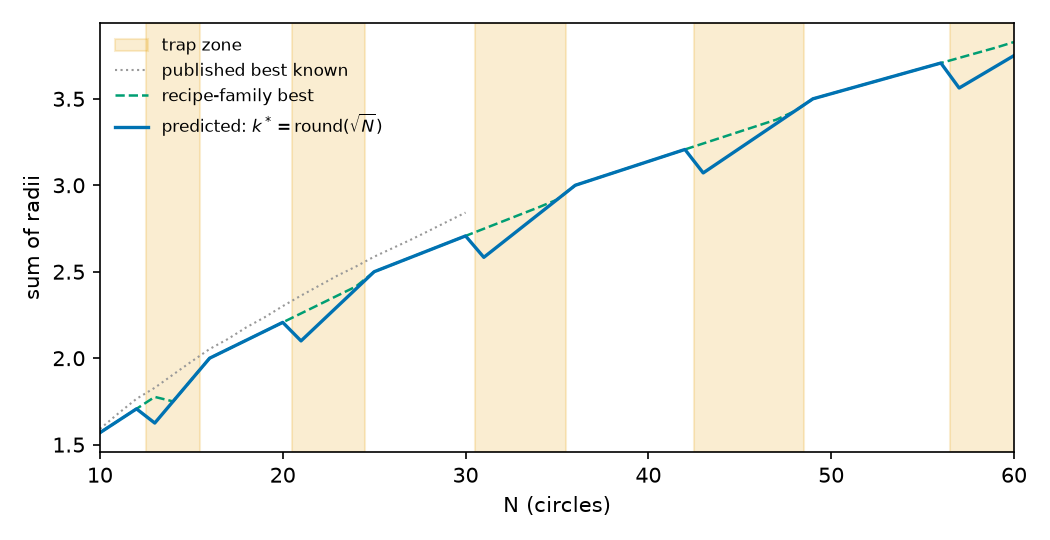
\includegraphics[width=\linewidth]{fig1_trapzones.png}
\caption{\emph{Predicted versus optimal value, $N = 10\ldots60$.} (i) the rule's prediction; (ii) the
best value in the recipe family; (iii, dotted) published best-known values \citep{friedman_packing}, terminating at
$N = 30$ because the bound table stops there. Shaded bands are the trap zones, the last being
$[57,63]$ clipped by \texttt{sweep(10,60)}. Worst-in-zone penalties 8.51\%, 7.03\%, 6.01\%, 5.25\%, 4.66\%; these are
family-internal arithmetic and exact at every $N$, while the published-bound comparison (curve iii)
is checkable only up to $N = 30$, where the bound table stops. The gap
closes to zero at $N = 35$ and $N = 48$ but \textbf{not} at $N = 24$, where 0.59\% remains --- curve (ii)
sits strictly above (i) across $[21,24]$.}
\label{fig:trapzones}
\end{figure}

\section{Task and recipe family}

\subsection{The benchmark}

Maximize the sum of radii of $N$ non-overlapping circles in the unit square. Feasibility is
decidable exactly from emitted coordinates, so proposals score with no human in the loop.

All invocations in the core arms are zero-shot and code-free. The prompt (Appendix A) fixes the
count, states containment and non-overlap, forbids writing or executing code, and demands only a
raw Python list of \texttt{[x, y, r]} triples. Our reason for the code-free design is that a code
channel routes the task to an executed optimizer, so the distribution would reflect the
optimizer. That reason is now measured rather than asserted: three preregistered code-channel
arms (\S3.7 --- weak tier, a fresh-draw replication, and a Sonnet-tier probe) find that
delegating construction to a math-only executed program neither escapes the family ceiling
(0 of 115 valid outputs above the argmax, across both tiers) nor dislodges the anchor as the
modal weak-tier output, so the code-free scope costs less loop relevance than we had
assumed --- with the library-assisted channel (\texttt{numpy}/\texttt{scipy}), the one
deployed loops permit, still unmeasured.

\subsection{The recipe family}

Three terms, used consistently: the \textbf{recipe family} is the parametric set of grid-plus-filler
constructions; a \textbf{template} is one member; the \textbf{anchor} is the template the distribution
concentrates on at a given $N$.

A $k \times k$ grid places one circle per cell center with $r_{\mathrm{grid}} = 1/(2k)$; $m$ fillers sit on interior
grid vertices, tangent to their four surrounding grid circles, with $r_{\mathrm{filler}} = (\sqrt{2} - 1)/(2k)$,
$0 \le m \le (k-1)^2$. Hence $V(k, m) = k/2 + m(\sqrt{2} - 1)/(2k)$. When $N < k^2$ the observed behavior is not
to drop to a smaller grid and fill it but to \emph{truncate} --- lay out the $k \times k$ lattice, occupy $N$
cells, leave the radius unchanged --- giving $T(k, N) = N/(2k)$. These reproduce every previously
reported anchor with no fitting: $V(5,1) = 2.5414214$, $V(5,2) = 2.5828427$, $V(5,0) = 2.500$,
$T(5,23) = 2.300$, $V(4,7) = 2.3624369$.

The finding that 94 of 95 valid proposals in prior arms were grid-plus-filler is retained only as
motivation, since those arms are not reported here; the self-contained version is \S5's
observation that across the 155 weak-tier rows collected before arm M only two exceeded the
family best, both by $\sim$$10^{-7}$ (arm M's 57 rows are scored separately in \S3.4 and were not swept
for this claim).

\subsection{The order rule is a definition; the branch rule is the hypothesis}

We write $k^*(N) = \lfloor \sqrt{N} + \tfrac{1}{2} \rfloor = \mathrm{round}(\sqrt{N})$ for the nearest-square order. This is a \emph{definition}. Given that the model emits some $k \times k$ grid from this family, ``the nearest
square lattice'' yields $\mathrm{round}(\sqrt{N})$ by construction; and $\arg\min_k |k^2 - N|$ switches at
$N = k^2 + k + \tfrac{1}{2}$ where $\mathrm{round}(\sqrt{N})$ switches at $k^2 + k + \tfrac{1}{4}$, so on the integers the two coincide
exactly --- two formalizations of ``nearest'' agreeing is a symptom that no substantive hypothesis
is being selected. Scoring four candidate orders against the three fitting anchors gave
\texttt{nearest} 3/3, \texttt{floor} 2/3, \texttt{argmax} 2/3, \texttt{ceil} 1/3; under a null where each candidate matches
each anchor with probability $\tfrac{1}{2}$, some candidate among four goes 3/3 about 40\% of the time, so
this is a weakly identified discrete selection, not a zero-parameter law.

The falsifiable content is the \textbf{branch rule}: $k^{*2} \le N \rightarrow$ extend with $m = N - k^{*2}$ fillers
(converge); $k^{*2} > N \rightarrow$ truncate the $k^*$-grid (trap). The extend arm survived testing only at
$m \le 1$ --- a preregistered extension disconfirmed it at $m \ge 4$, where the model prefers the
$(k^*{+}1)$ rectangle grid (\S3.4). Nothing about ``nearest'' forces truncation ---
a proposer with any local search would drop to $k^*{-}1$ and fill, which is why the trap zones exist
and why a higher-valued rival is reachable inside them. Truncate-versus-drop-and-fill is a
genuine dichotomy, and it is what \S3 and \S4 test. The governing quantity is the signed distance
$N - k^{*2}$. Primality is not the variable --- 13, 23, 31, 43, 47 and 59 trap while 11, 17, 19, 29,
37, 41 and 53 converge --- refuting the prior work's conjecture about primes near 30 before any
model is queried.

\subsection{Notation and conventions}

Terms used throughout, gathered here so no verdict table depends on a definition made
elsewhere:

\begin{center}
\begin{small}
\begin{tabular}{@{}p{0.26\linewidth}p{0.68\linewidth}@{}}
\toprule
Term & Meaning \\
\midrule
$k^*(N)$ & nearest-square grid order, $\mathrm{round}(\sqrt{N})$ (a definition, \S2.3) \\
$V(k, m)$, $T(k, N)$ & extend-with-$m$-fillers value $k/2 + m(\sqrt{2}-1)/(2k)$; truncated-grid value $N/(2k)$ \\
anchor & the template the proposal distribution concentrates on at a given $N$ \\
attractor & the same object, used when the emphasis is on the family a tier converges to rather than on one cell (\S5) \\
on-prediction & emitted sum within $2\times10^{-3}$ of the registered predicted value \\
rival (argmax) & the highest-valued member of the recipe family at that $N$ when it differs from the prediction --- inside a trap zone, $V(k^*{-}1, m)$ \\
discriminating cell & $N$ where prediction $\ne$ family argmax; only these can distinguish anchoring from family search \\
validity & non-overlap and containment at $10^{-6}$ (primary) and $10^{-9}$ (logged), both always reported \\
trap / converge & branch by sign of $N - k^{*2}$: truncate when $k^{*2} > N$, extend when $k^{*2} \le N$ \\
tier & nominal capability class of the serving alias addressed (weak/mid/top); \texttt{opus\_alias} is a bare alias with no attestable weights binding \\
BELOW-FLOOR & model failing its arm's registered validity floor; no anchoring claim in either direction \\
UNSCOREABLE & cell with $<$ 3 valid samples under the GM-chain registration; claims nothing \\
mixed-serving accounting & pooled rate including cells collected through a registered serving-path amendment; the first-party-only rate is always given beside it \\
\bottomrule
\end{tabular}
\end{small}
\end{center}
